\documentclass{article}
\usepackage{graphicx}
\graphicspath{ {.} }
\usepackage[backend=biber]{biblatex}
\addbibresource{report.bib}

\usepackage[T1]{fontenc}

\usepackage{amsmath}

\usepackage{url}

\author{Yash Malviya 2016CS50403 \\ Aniket Kumar 2016CS50397}

\title{Accelerating Matrix Multiplication}
\date{February 17, 2019}

\begin{document}
\maketitle

\section{Linear Algebra Libraries}

The following was done to speed up convolution process 
required for solving Digit Recognition Problem using 
Convolutional Nueral Networks. 

Convolution is done by converting the image and kernel 
into corresponding Toeplitz matrices
(\textcite{wiki:toepliz}).

Function from Basic Linear Algebra Subprograms used 
\textbf{cblas\_sgemm}. Which perform following 
mathematical operation.

\begin{math}
    C \Leftarrow \alpha A*B + \beta C
\end{math}

where A is processed Toeplitz image matrix,
B is processed kernel column vector, 
C is zero matrix and 
\begin{math}
    \alpha(=1.0)\ and\ \beta(=0.0)\ are\ constants.
\end{math}

\subsection{OpenBLAS}

\emph{Open source} implementation of the 
Basic Linear Algebra Subprograms: \textcite{OpenBLAS:wiki} 

\subsection{Intel MKL}

\emph{Intel}'s Math Kernel Library, another 
implementation of BLAS: \textcite{IntelMKL:doc}

\section{Performance comparison}
We get a increase in performance of calculating matrix convolution using these libraries.
Intel MKL library give best performance among all these implementations.\newline
As size of input matrix increases, time taken by PThread tends to time taken by IntelMKL library.\newline
The comparison of performance of the three implementations(OpenBLAS , MKL and PThread) are shown as below :
\begin{figure}
  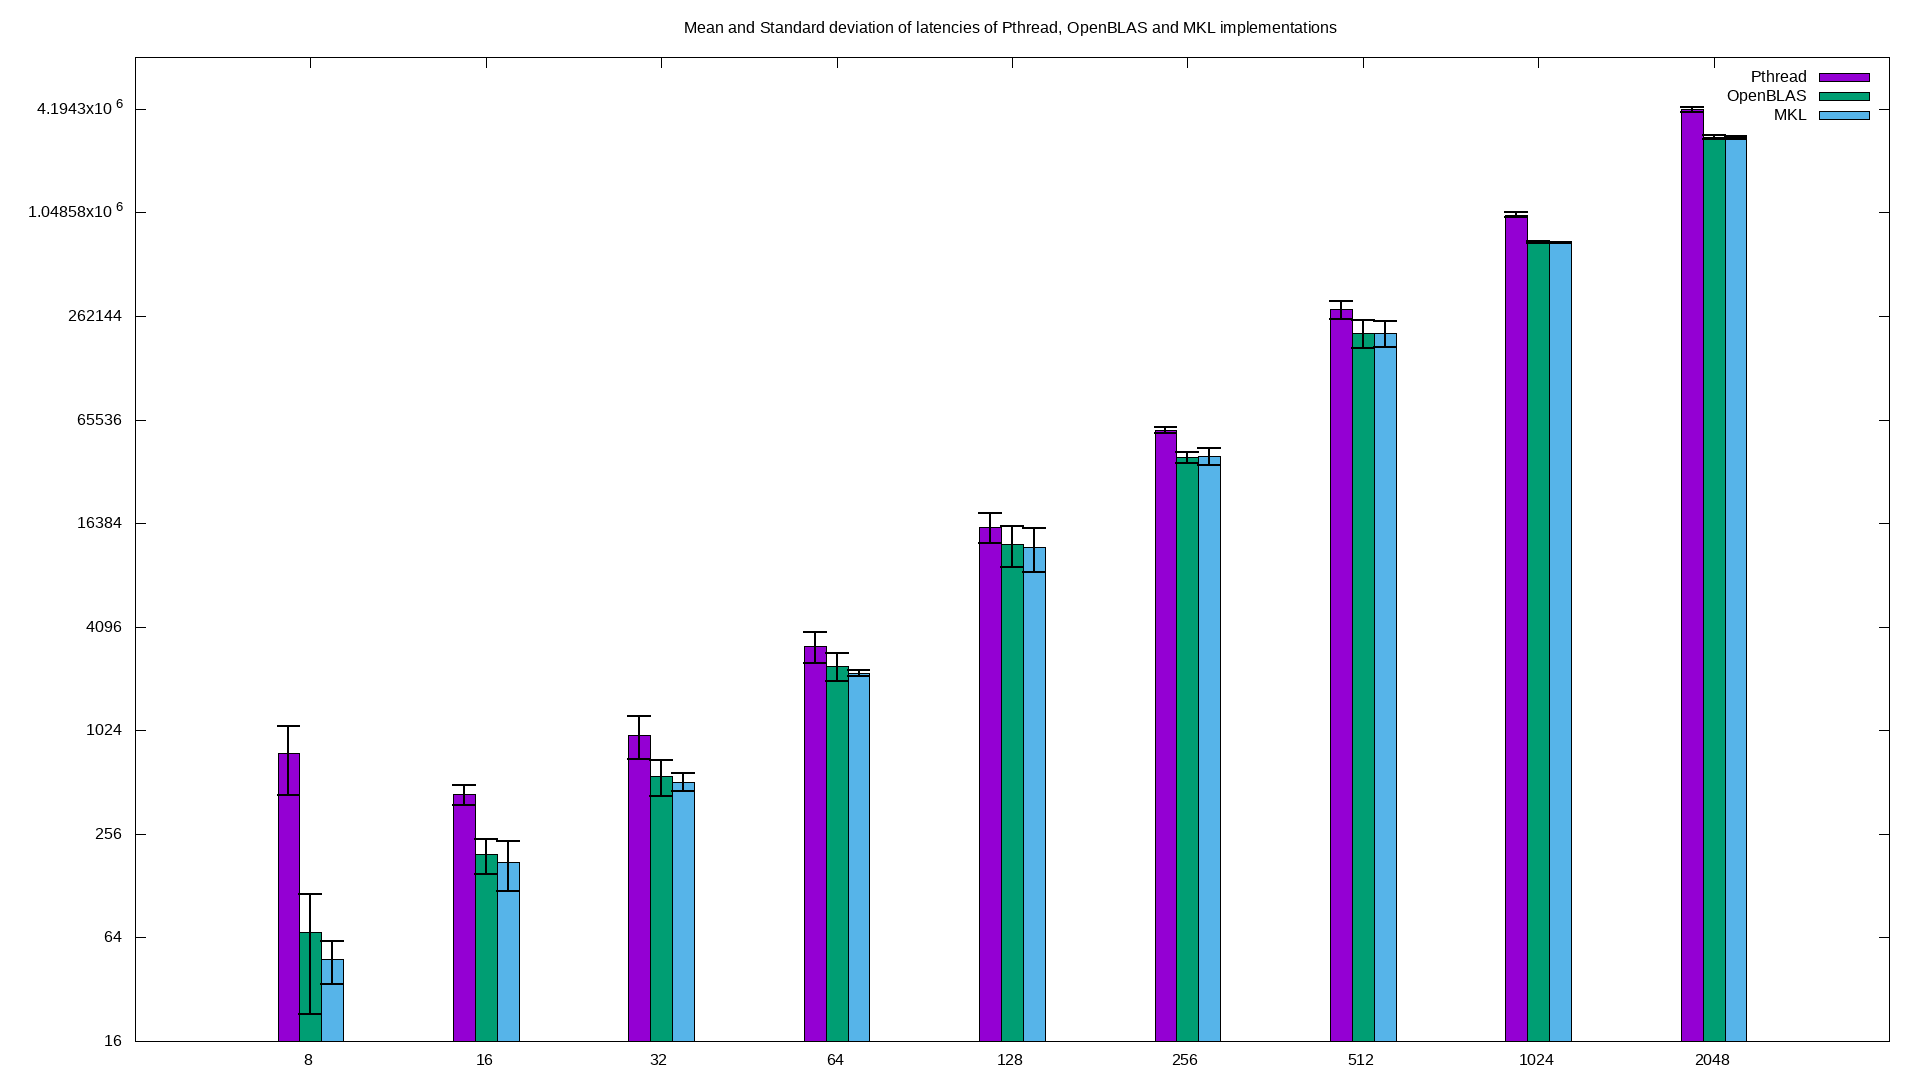
\includegraphics[width=\linewidth]{performance.png}
  \caption{Plot of time V/S Matrix Size in different implementations}
%   \label{fig:}
\end{figure}

\section{Acceleration with pthreads}

\subsection{Parallelization Stratergy}

\begin{itemize}
    \item Inner product of row of A and the column vector B 
    is done by each thread.

    \item Each thread gets the row it operates on, in a 
    round robin fashion. 
    
    \textit{For Ex:} say there are k threads, then thread with 
    tid 0 gets 1\textsuperscript{st} row, k+1\textsuperscript{th} 
    row 2k+1\textsuperscript{th} row and so on.


\end{itemize}

\subsection{Difficulties encountered}

\begin{enumerate}
    \item Writing to only different sections of 
    shared memory space.
    \item Ensuring all shared memory which was 
    allocated on heap doesn't leak.
    \item Passing thread ID to each thread 
    through shared space. 
\end{enumerate}

\printbibliography

\end{document}
